\begin{figure}[H]
\centering
\shorthandoff{<>}
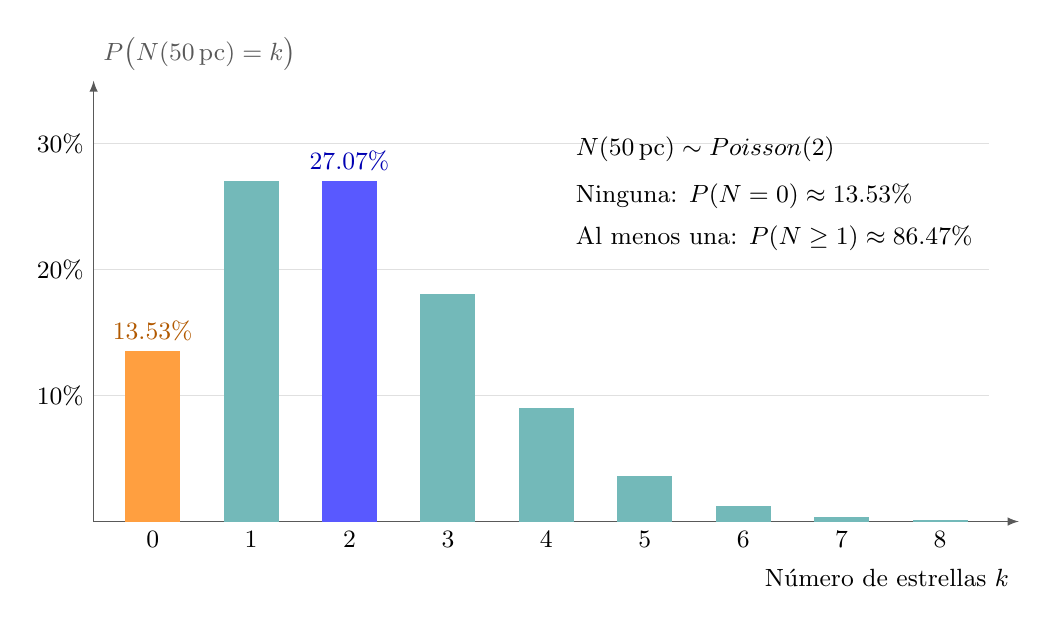
\begin{tikzpicture}[x=1.25cm,y=0.16cm,font=\small,>=latex]
  \foreach \level in {10,20,30}{
    \draw[black!12] (-0.6,\level) -- (8.5,\level);
    \node[left] at (-0.6,\level) {$\level\%$};
  }
  \draw[->,black!65] (-0.6,0) -- (8.8,0);
  \draw[->,black!65] (-0.6,0) -- (-0.6,35)
    node[above right] {$P\bigl(N(50\,\mathrm{pc})=k\bigr)$};
  \foreach \countvalue/\probability in {0/13.5335,1/27.0671,2/27.0671,3/18.0447,4/9.0224,5/3.6089,6/1.2030,7/0.3437,8/0.0859}{
    \fill[teal!55] ({\countvalue-0.28},0) rectangle ({\countvalue+0.28},\probability);
    \node[below] at (\countvalue,0) {$\countvalue$};
  }
  \fill[orange!75] (-0.28,0) rectangle (0.28,13.5335);
  \fill[blue!65] (1.72,0) rectangle (2.28,27.0671);
  \node[above,text=orange!70!black] at (0,13.5335) {$13.53\%$};
  \node[above,text=blue!70!black] at (2,27.0671) {$27.07\%$};
  \node[align=left,anchor=west] at (4.2,26)
    {$N(50\,\mathrm{pc})\sim\operatorname{Poisson}(2)$\\[6pt]
     Ninguna: $P(N=0)\approx13.53\%$\\[4pt]
     Al menos una: $P(N\ge1)\approx86.47\%$};
  \node[anchor=north east] at (8.8,-3) {Número de estrellas $k$};
\end{tikzpicture}
\shorthandon{<>}
\caption{Probabilidades del conteo en un segmento de $50\,\mathrm{pc}$. La barra naranja representa ninguna estrella y la azul, exactamente dos. El evento ``al menos una'' reúne todas las barras con $k\ge1$, incluida la azul. Se muestran los conteos hasta $8$; los valores superiores conservan una pequeña probabilidad. Al ser una distribución discreta, cada probabilidad corresponde a la altura de su barra.}
\label{fig:poisson-conteo}
\end{figure}